\section{Parte 4: del AR(1) al SARIMA}
\label{sec:parte4}

Se sigue la receta del enunciado: quitar la estacionalidad, mirar el residuo
y modelar la memoria que quede. Toda la parte usa los 245 días abiertos del
entrenamiento como una fila por día. El código está en \texttt{parte4.py} y la
configuración de S1 y S2 en \texttt{modelos.py}, que se reusa en la Parte~5.

\subsection{Inciso 4.1: quitar el día de la semana}

Se ajusta por OLS $y_t = \sum_{d} \beta_d D_{d,t} + e_t$, con una indicadora
$D_{d,t}$ por cada uno de los seis días abiertos y sin intercepto. Con esa
especificación, cada $\hat\beta_d$ es simplemente la venta promedio de ese día
de la semana: lunes \pounds26\,916, martes \pounds34\,988, miércoles
\pounds27\,695, jueves \pounds35\,266, viernes \pounds26\,208 y domingo
\pounds13\,706. El mismo orden que los índices estacionales del inciso 3.2.

\begin{figure}[H]
  \centering
  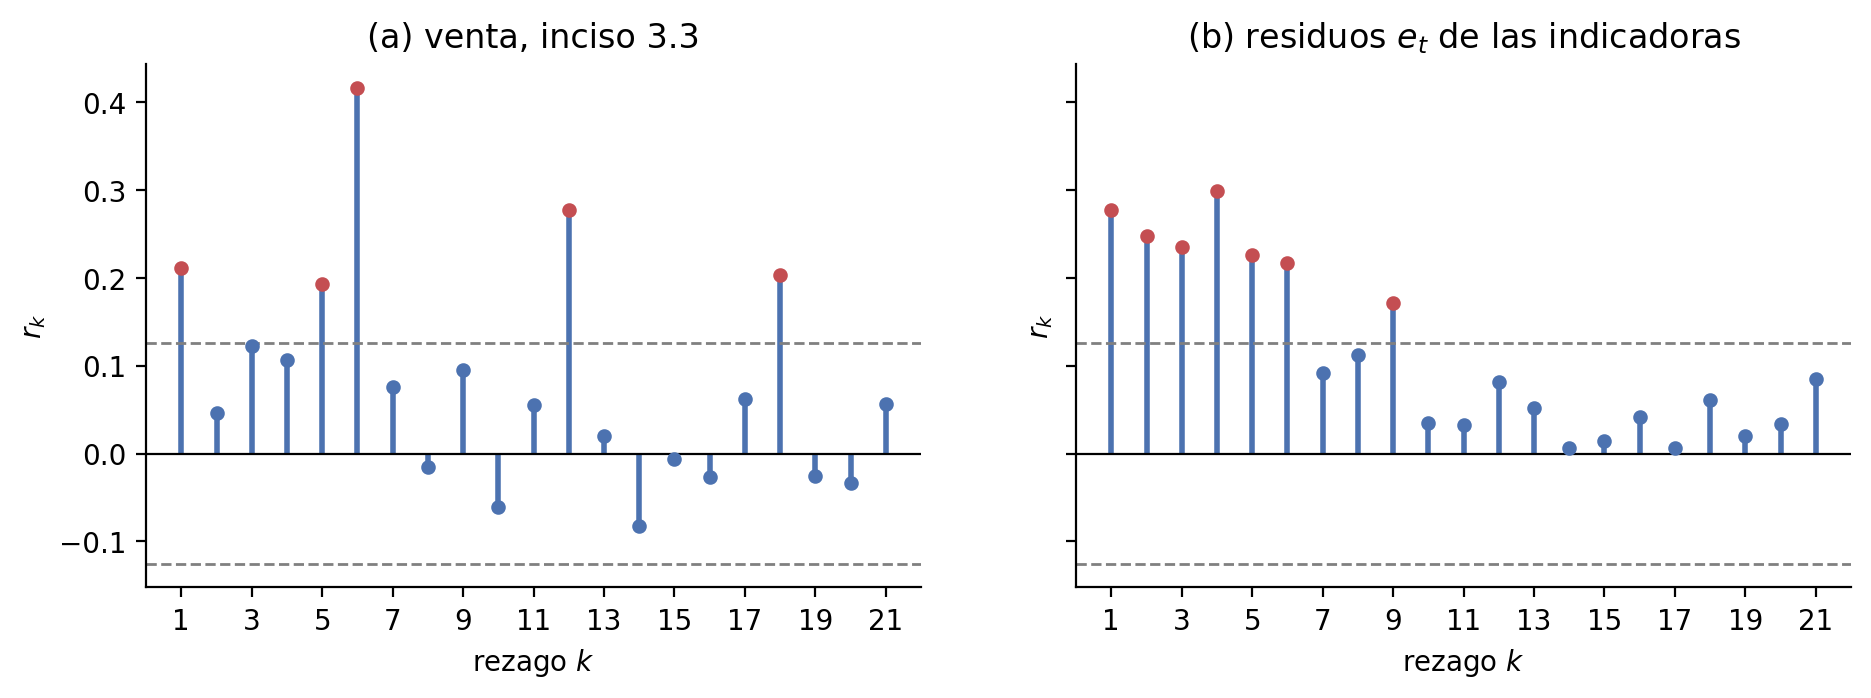
\includegraphics[width=\textwidth]{p4_acf_indicadoras.png}
  \caption{ACF antes (a) y después (b) de quitar el efecto del día de la
  semana, con las mismas bandas $\pm1.96/\sqrt{245}$.}
  \label{fig:p4_acf_ind}
\end{figure}

\paragraph{¿Qué cambió respecto a 3.3?} Los picos en 6, 12 y 18
desaparecieron: $r_{12}$ y $r_{18}$ de los residuos ya están dentro de las
bandas, y $r_6$ bajó de 0.42 a 0.22, al nivel de los rezagos vecinos
(figura~\ref{fig:p4_acf_ind}). Las indicadoras se llevaron el patrón semanal,
que era media no constante, tal como se había anticipado en 3.3(b). Pero lo
que queda no es ruido blanco: los nueve primeros rezagos son positivos y
están fuera de las bandas (salvo el 7 y el 8, que quedan cerca), entre 0.17 y
0.30, y la ACF baja lentamente hasta desaparecer después del rezago 10.
Ljung--Box es todavía mayor que antes ($Q(6)=95.2$; tabla~\ref{tab:p4_lb}).

\paragraph{¿Se parece a un AR(1) o al proceso con tendencia?} Un AR(1) con
$\phi\approx0.28$ (el $r_1$ de los residuos) tendría $r_2\approx0.08$ y
$r_4\approx0.006$: una caída geométrica rápida. Aquí $r_2=0.25$, $r_3=0.24$ y
$r_4=0.30$; la ACF casi no decae en los primeros seis rezagos. Esa es la forma
de la ACF del proceso con tendencia de la Parte 0 (tabla~\ref{tab:p0_sin_memoria}),
donde $r_1$, $r_5$ y $r_7$ eran todos parecidos. El residuo de la
figura~\ref{fig:p4_res} muestra por qué: es positivo casi todo diciembre de
2010 y septiembre de 2011, y negativo casi todo de enero a abril. Los días
vecinos comparten el signo porque comparten el nivel.

\begin{figure}[H]
  \centering
  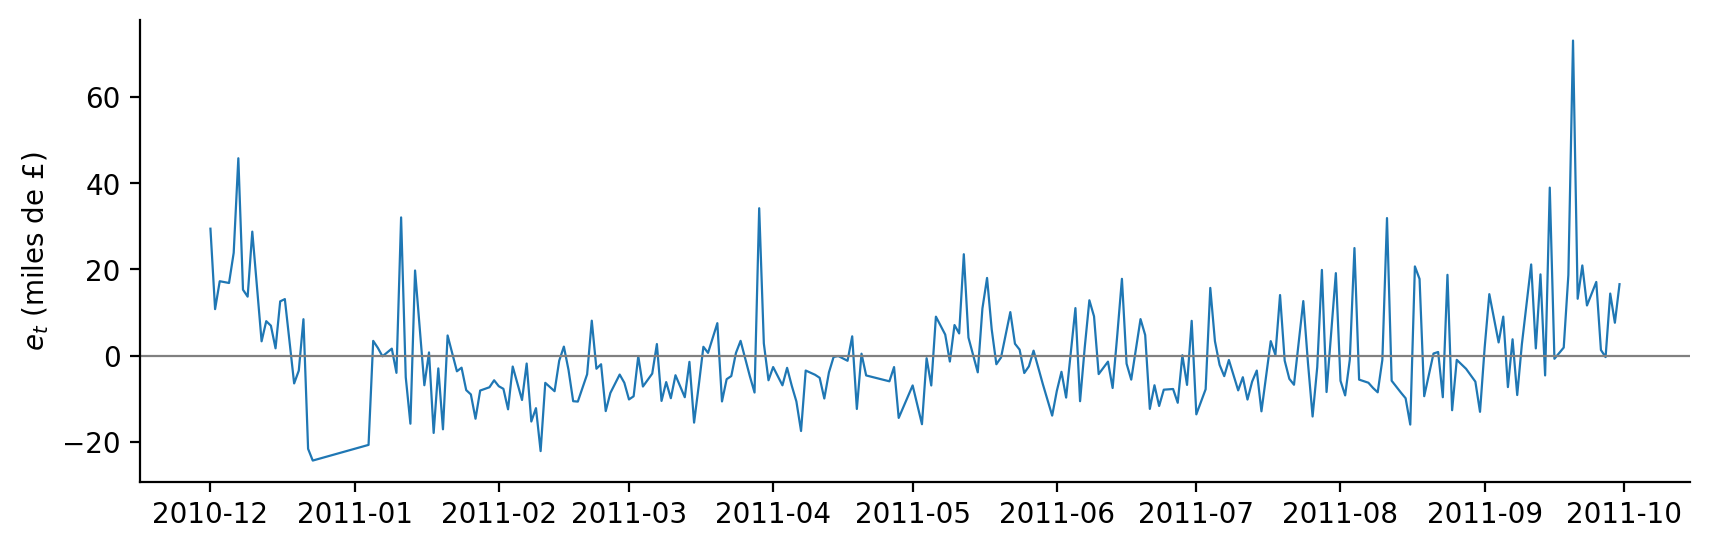
\includegraphics[width=\textwidth]{p4_residuos_indicadoras.png}
  \caption{Residuos $e_t$ de la regresión contra las indicadoras de día de la
  semana.}
  \label{fig:p4_res}
\end{figure}

\paragraph{¿Qué le falta al modelo?} Le falta el nivel. Las indicadoras
suponen que un martes de febrero y un martes de septiembre tienen la misma
media, pero la serie cambia de nivel (inciso 3.1): baja en enero, queda plana
y sube desde septiembre. Ese nivel que se mueve es media no constante que el
modelo no tiene, y queda en los residuos como autocorrelación positiva en
todos los rezagos cortos.

\subsection{Inciso 4.2: un AR(1) sobre los residuos}

Se ajusta por OLS $e_t = c + \phi e_{t-1} + u_t$ y se obtiene
$\hat\phi=0.279$ (con $\hat c=-101.7$, prácticamente cero, como corresponde a
residuos de media cero). La figura~\ref{fig:p4_acf_ar1} es la ACF de
$u_t=e_t-\hat c-\hat\phi e_{t-1}$.

\begin{figure}[H]
  \centering
  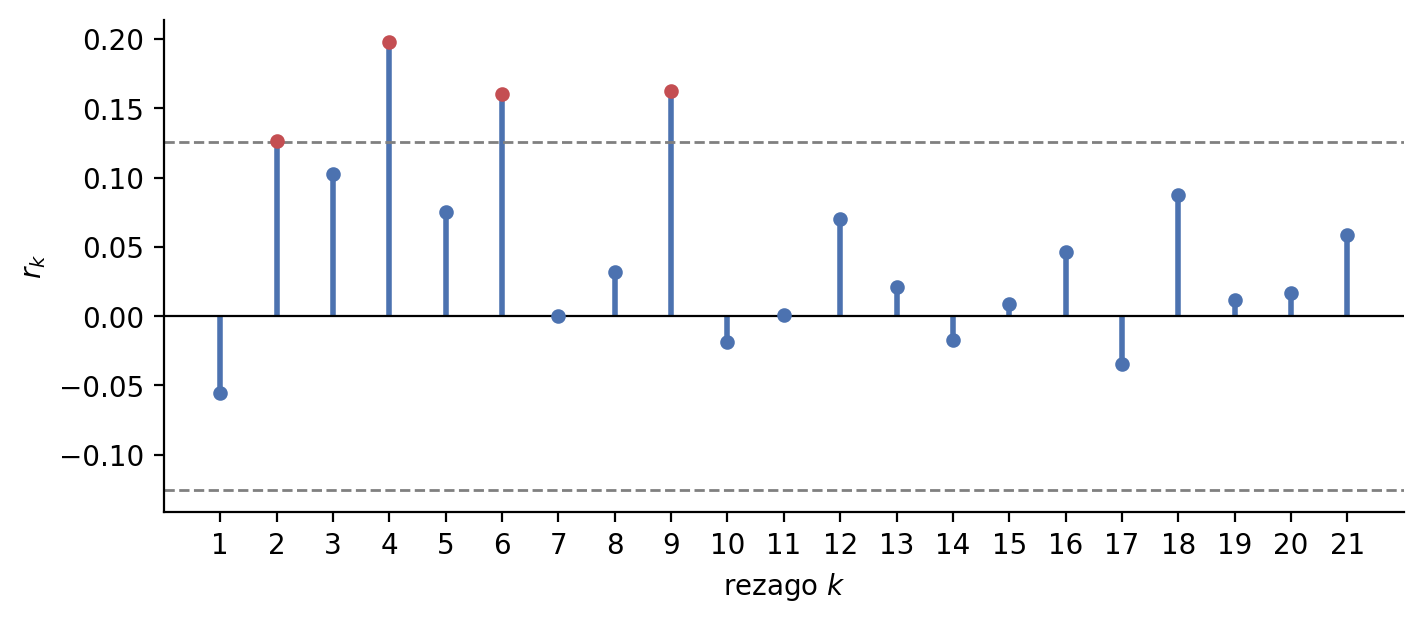
\includegraphics[width=0.8\textwidth]{p4_acf_ar1.png}
  \caption{ACF de los residuos $u_t$ del AR(1) ajustado a $e_t$.}
  \label{fig:p4_acf_ar1}
\end{figure}

\begin{table}[H]
  \centering
  \small
  \tabla{p4_ljungbox}
  \caption{Ljung--Box sobre los residuos de cada etapa. Los grados de
  libertad restan los parámetros de memoria estimados: uno para el AR(1) y
  dos para S1 y S2.}
  \label{tab:p4_lb}
\end{table}

Todavía no son ruido blanco. El AR(1) se llevó el rezago 1 ($r_1$ pasó de
0.28 a $-0.06$), pero siguen fuera de las bandas los rezagos 2, 4, 6 y 9
($r_4=0.20$, $r_6=0.16$, $r_9=0.16$). Ljung--Box lo confirma: $Q(6)=25.1$ con 5
grados de libertad y $Q(12)=33.4$ con 11, con valores-$p$ de $10^{-4}$. Un
AR(1) no alcanzó, y era de esperarse: el AR(1) modela una memoria que se
desvanece geométricamente, y lo que había en 4.1 era un nivel que se mueve
durante meses. El AR(1) solo puede representarlo como ``hoy se parece a
ayer'', y por eso arregla el rezago 1 y deja el resto.

\subsection{Inciso 4.3: SARIMA}

Con \texttt{statsmodels.tsa.statespace.sarimax.SARIMAX} se ajustan, sobre
$\log y_t$, los dos modelos con $s=6$:
\begin{align*}
  \text{S1:}\quad & (1-\phi B)(1-\Phi B^6)(\log y_t - \mu) = \varepsilon_t,
    \qquad\text{SARIMA}(1,0,0)(1,0,0)_6 \text{ con constante;}\\
  \text{S2:}\quad & (1-B)(1-B^6)\log y_t = (1+\theta B)(1+\Theta B^6)\varepsilon_t,
    \qquad\text{SARIMA}(0,1,1)(0,1,1)_6 \text{ sin constante.}
\end{align*}
A \texttt{SARIMAX} se le pasa el arreglo de valores, no la serie con fechas.
En \texttt{statsmodels} la constante de S1 se estima como el intercepto $c$
de la ecuación, que se relaciona con la media por
$c=\mu(1-\phi)(1-\Phi)$.

\paragraph{¿Por qué $s=6$ y no 7?} Porque el modelo trabaja con una fila por
día abierto, y una semana tiene seis días abiertos: el martes anterior está
seis filas atrás, no siete (el pico de la ACF del inciso 3.3 estaba en 6). Con
$s=7$ el modelo compararía cada día con un día de la semana distinto cada vez.

\paragraph{¿Cuándo se rompe esa suposición?} Cuando una semana tiene menos de
seis días abiertos. Después de un feriado, seis filas atrás ya no es el mismo
día de la semana: después del Lunes de Pascua (25 de abril), por ejemplo, las
filas quedan desfasadas un día durante una semana, y el modelo compara un
martes con un miércoles. El caso extremo es el cierre de Navidad, que se come
nueve días. Según el inciso 3.3, 28 de los 239 pares de días a distancia 6 no
están a una semana; en esos puntos la estacionalidad del modelo apunta al día
equivocado.

\paragraph{¿Por qué el logaritmo?} Porque la variación de la serie crece con
su nivel. En febrero la venta diaria promedia \pounds20.7 mil con una
desviación estándar de \pounds8.5 mil; en septiembre promedia \pounds38.9 mil
y la desviación sube a \pounds18.9 mil. En logaritmo, la desviación estándar
mensual queda entre 0.35 y 0.69 durante todo el año, sin crecer con el
nivel. Además, los índices
estacionales del inciso 3.2 son multiplicativos: el martes vende un 55\% más
que su semana, no una cantidad fija de libras más. FPP2 (§3.2) recomienda
transformar cuando la variación depende del nivel. El logaritmo convierte la
estructura multiplicativa en aditiva, $\log y_t = \log T_t + \log S_t + \log
R_t$, que es lo que un SARIMA sabe modelar, y estabiliza la varianza. Además
garantiza que el pronóstico en libras, $\exp(\cdot)$, sea positivo. Se puede
usar porque en los días abiertos la venta neta es siempre positiva: el mínimo
del entrenamiento es \pounds3\,440.

\paragraph{Convergencia.} La tabla~\ref{tab:p4_sarima} muestra los
parámetros con el límite de iteraciones por defecto (50) y con 500.

\begin{table}[H]
  \centering
  \small
  \tabla{p4_sarima}
  \caption{Parámetros de S1 y S2 sobre $\log y_t$ con 50 y 500 iteraciones
  como máximo. ``Convergió'' es \texttt{mle\_retvals['converged']}.}
  \label{tab:p4_sarima}
\end{table}

S2 converge en 14 iteraciones y sus parámetros no cambian al subir
\texttt{maxiter}. S1 \emph{no} converge con el valor por defecto: se detiene en
la iteración 50 con $\Phi=0.906$, $\phi=0.164$ y $c=0.795$. Con
\texttt{maxiter=500} converge en 81 iteraciones a un modelo distinto:
$\Phi=0.521$, $\phi=0.132$ y $c=4.210$, con una log-verosimilitud mucho
mayor ($-160.7$ contra $-185.9$). Lo interesante es que los dos conjuntos de
parámetros implican casi la misma media, $\mu=c/((1-\phi)(1-\Phi))\approx
10.12$ en logaritmo, es decir, \pounds24\,900 diarios. Lo que cambia es la
dinámica: el optimizador sin terminar estaba en una región con $\Phi$ cerca
de 1, casi una raíz unitaria estacional, que es un modelo con mucha más
memoria semanal de la que tienen los datos. Sin revisar
\texttt{mle\_retvals} se habría usado ese modelo sin saberlo. De aquí en
adelante S1 se ajusta siempre con \texttt{maxiter=500}.

\subsection{Inciso 4.4: diagnóstico}

Los residuos de S2 empiezan con valores enormes ($10.9$ en el primero y
$-6.1$ en el séptimo, cuando los demás son del orden de $\pm0.5$): con
inicialización difusa, las primeras $1+6=7$ observaciones solo sirven para
arrancar las diferencias $(1-B)(1-B^6)$ y sus residuos no significan nada. Se
descartan. La figura~\ref{fig:p4_acf_sarima} y la tabla~\ref{tab:p4_lb}
muestran el resultado, con $m-2$ grados de libertad.

\begin{figure}[H]
  \centering
  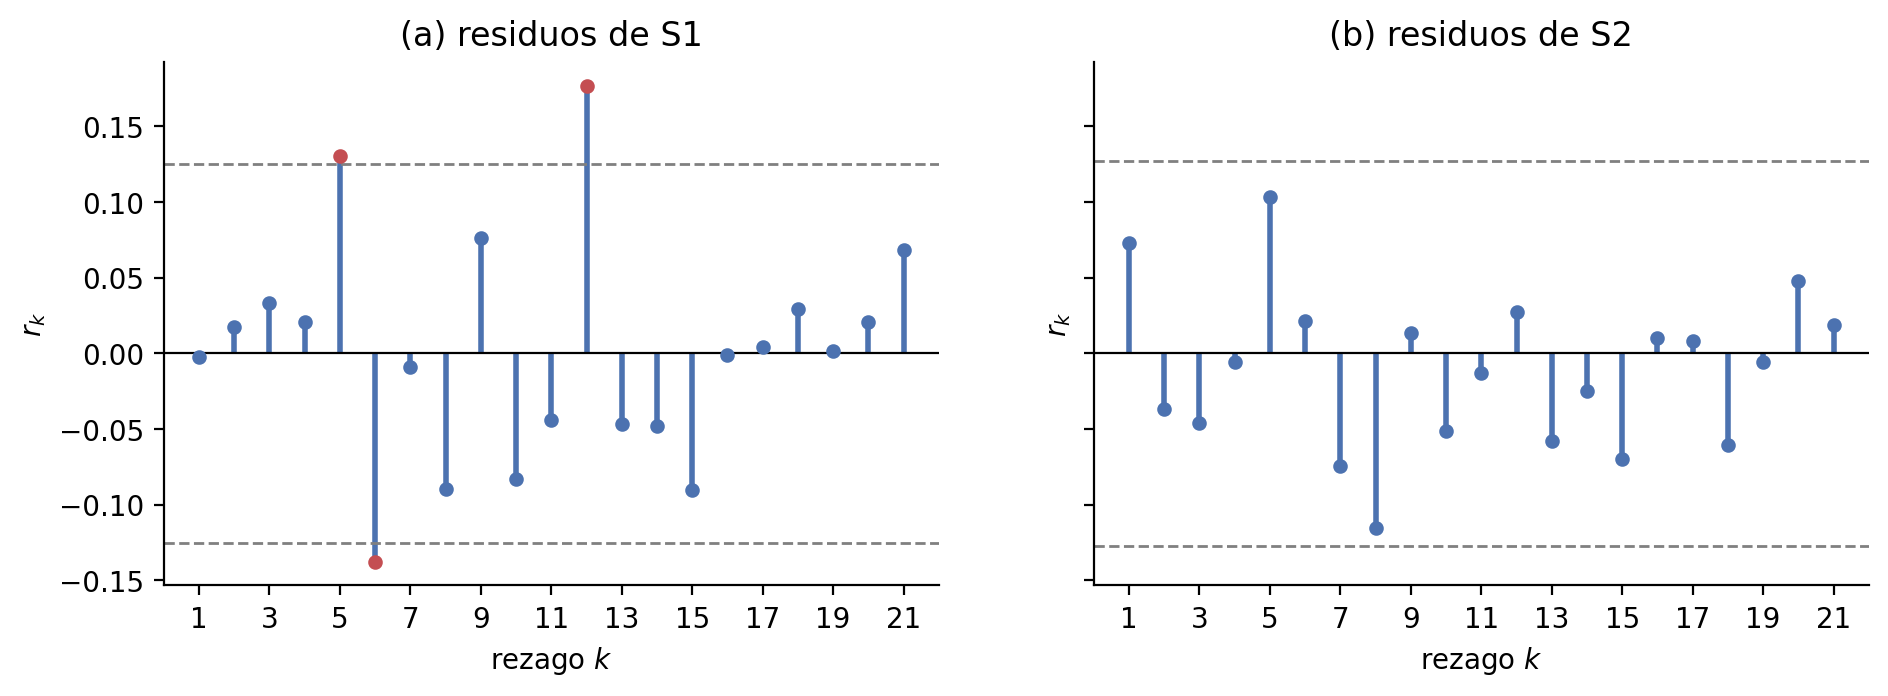
\includegraphics[width=\textwidth]{p4_acf_sarima.png}
  \caption{ACF de los residuos de S1 (con \texttt{maxiter=500}) y de S2 (sin
  sus primeros 7 residuos).}
  \label{fig:p4_acf_sarima}
\end{figure}

\begin{itemize}
  \item \textbf{S1 no deja ruido blanco.} $Q(6)=9.5$ con 4 grados de
    libertad ($p=0.049$, justo en la frontera) y $Q(12)=23.5$ con 10
    ($p=0.009$): se rechaza ruido blanco. S1 modela la memoria y el patrón
    semanal, pero alrededor de una media \emph{fija}, y el cambio de nivel que
    se vio en 4.1 sigue en sus residuos.
  \item \textbf{S2 sí.} $Q(6)=4.9$ ($p=0.30$) y $Q(12)=10.5$ ($p=0.40$):
    no hay evidencia de autocorrelación en sus residuos. La diferencia
    $(1-B)$ es lo que le permite seguir un nivel que se mueve, y $(1-B^6)$
    se lleva el patrón semanal.
\end{itemize}

\subsection{Inciso 4.5: hacia dónde van los pronósticos}

La figura~\ref{fig:p4_horizonte} muestra los pronósticos de los dos modelos,
ajustados con todo el entrenamiento, para los siguientes 120 días abiertos.

\begin{figure}[H]
  \centering
  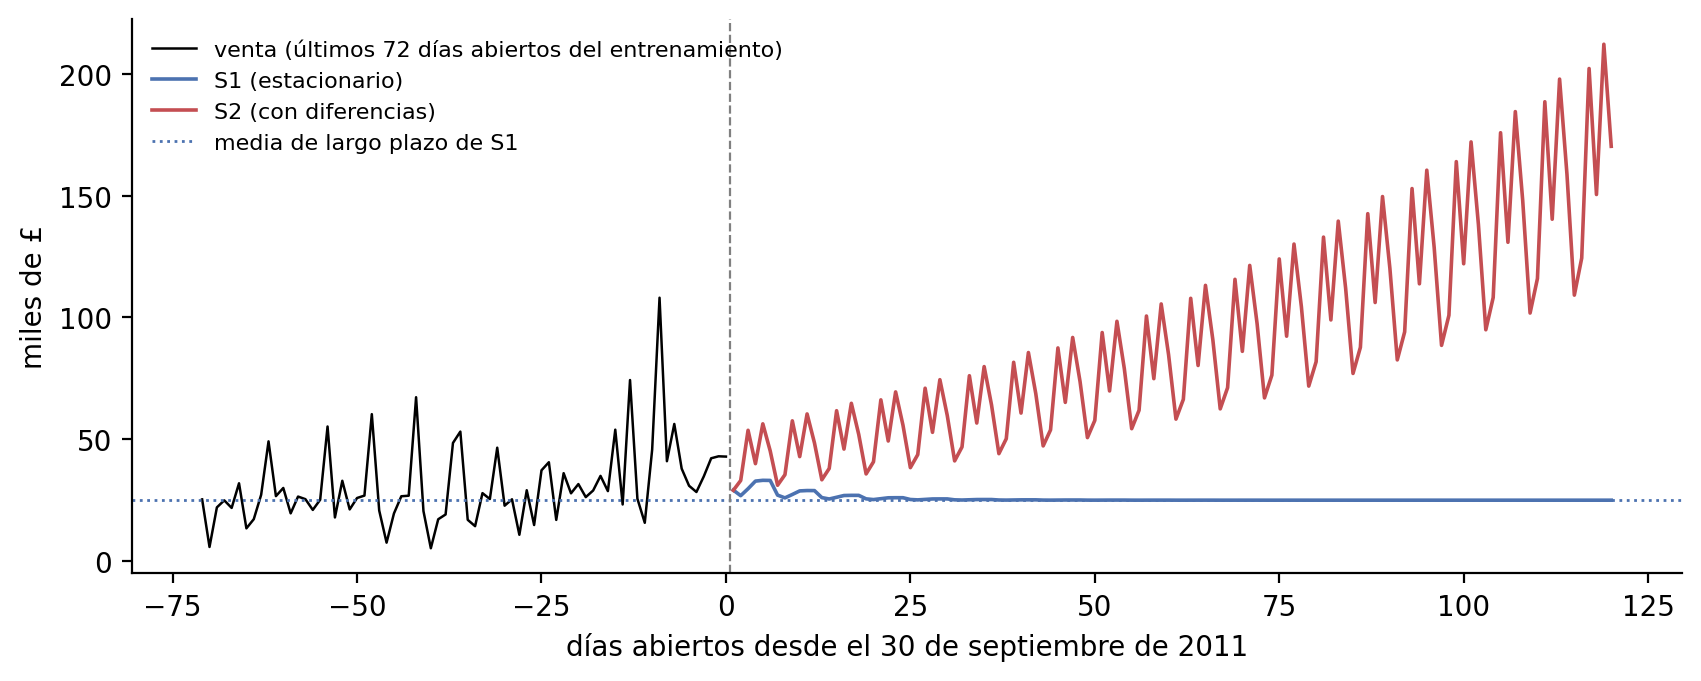
\includegraphics[width=\textwidth]{p4_horizonte.png}
  \caption{Pronósticos de S1 y S2 hasta 120 días abiertos después del 30 de
  septiembre de 2011, en libras ($\exp$ del pronóstico en logaritmo).}
  \label{fig:p4_horizonte}
\end{figure}

\paragraph{S1 regresa a su media.} Es estacionario, y en un AR estacionario el
efecto de lo observado decae como $\phi^h$ (inciso 0.1). Para S1 las dos
memorias, $\phi^h$ con $\phi=0.13$ y $\Phi^{h/6}$ con $\Phi=0.52$, se
desvanecen en unas pocas semanas, y el pronóstico converge a
$\exp(\mu)\approx$ \pounds24\,875 diarios, la venta típica de enero a
septiembre. A partir de un mes de horizonte, S1 pronostica lo mismo para
todos los días: ni siquiera conserva el patrón semanal, porque ese patrón
también lo modelaba como memoria que se desvanece.

\paragraph{S2 no regresa a ningún lado.} Igual que la caminata aleatoria, que
nunca olvida, S2 no tiene una media a la cual volver: su pronóstico arranca
del último nivel observado y conserva el último patrón semanal. Y como tiene
dos diferencias ($d=1$ y $D=1$), el pronóstico admite además una pendiente: la
estima con el promedio reciente de los cambios, y el crecimiento de septiembre
la hace positiva, así que la proyecta sin límite. A 120 días abiertos el
pronóstico supera las \pounds200 mil diarias. A horizontes cortos, ese
comportamiento es justo lo que S1 no puede hacer (seguir un nivel nuevo); a
horizontes largos, una extrapolación así es peligrosa. Para un pronóstico de
una semana, que es lo que pide la Parte 5, lo que importa es el corto plazo.
